
\chapter{Результаты}\label{chapt_results}
В результате полугода работы прибора ДЭПРОН накоплен большой массив информации - 25 тысяч файлов бинарных данных, общим объемом 100 МБайт. Первичные данные были распакованы и сохранены в текстовом виде.
Далее информация прибора ДЭПРОН была визуализирована с помошью пакета \texttt{lattice} и базовой графической системы R. На рисунке \ref{fig:depronseclog08-29-16} показаны результаты визуализации.
\begin{figure}[h]
	\centering
	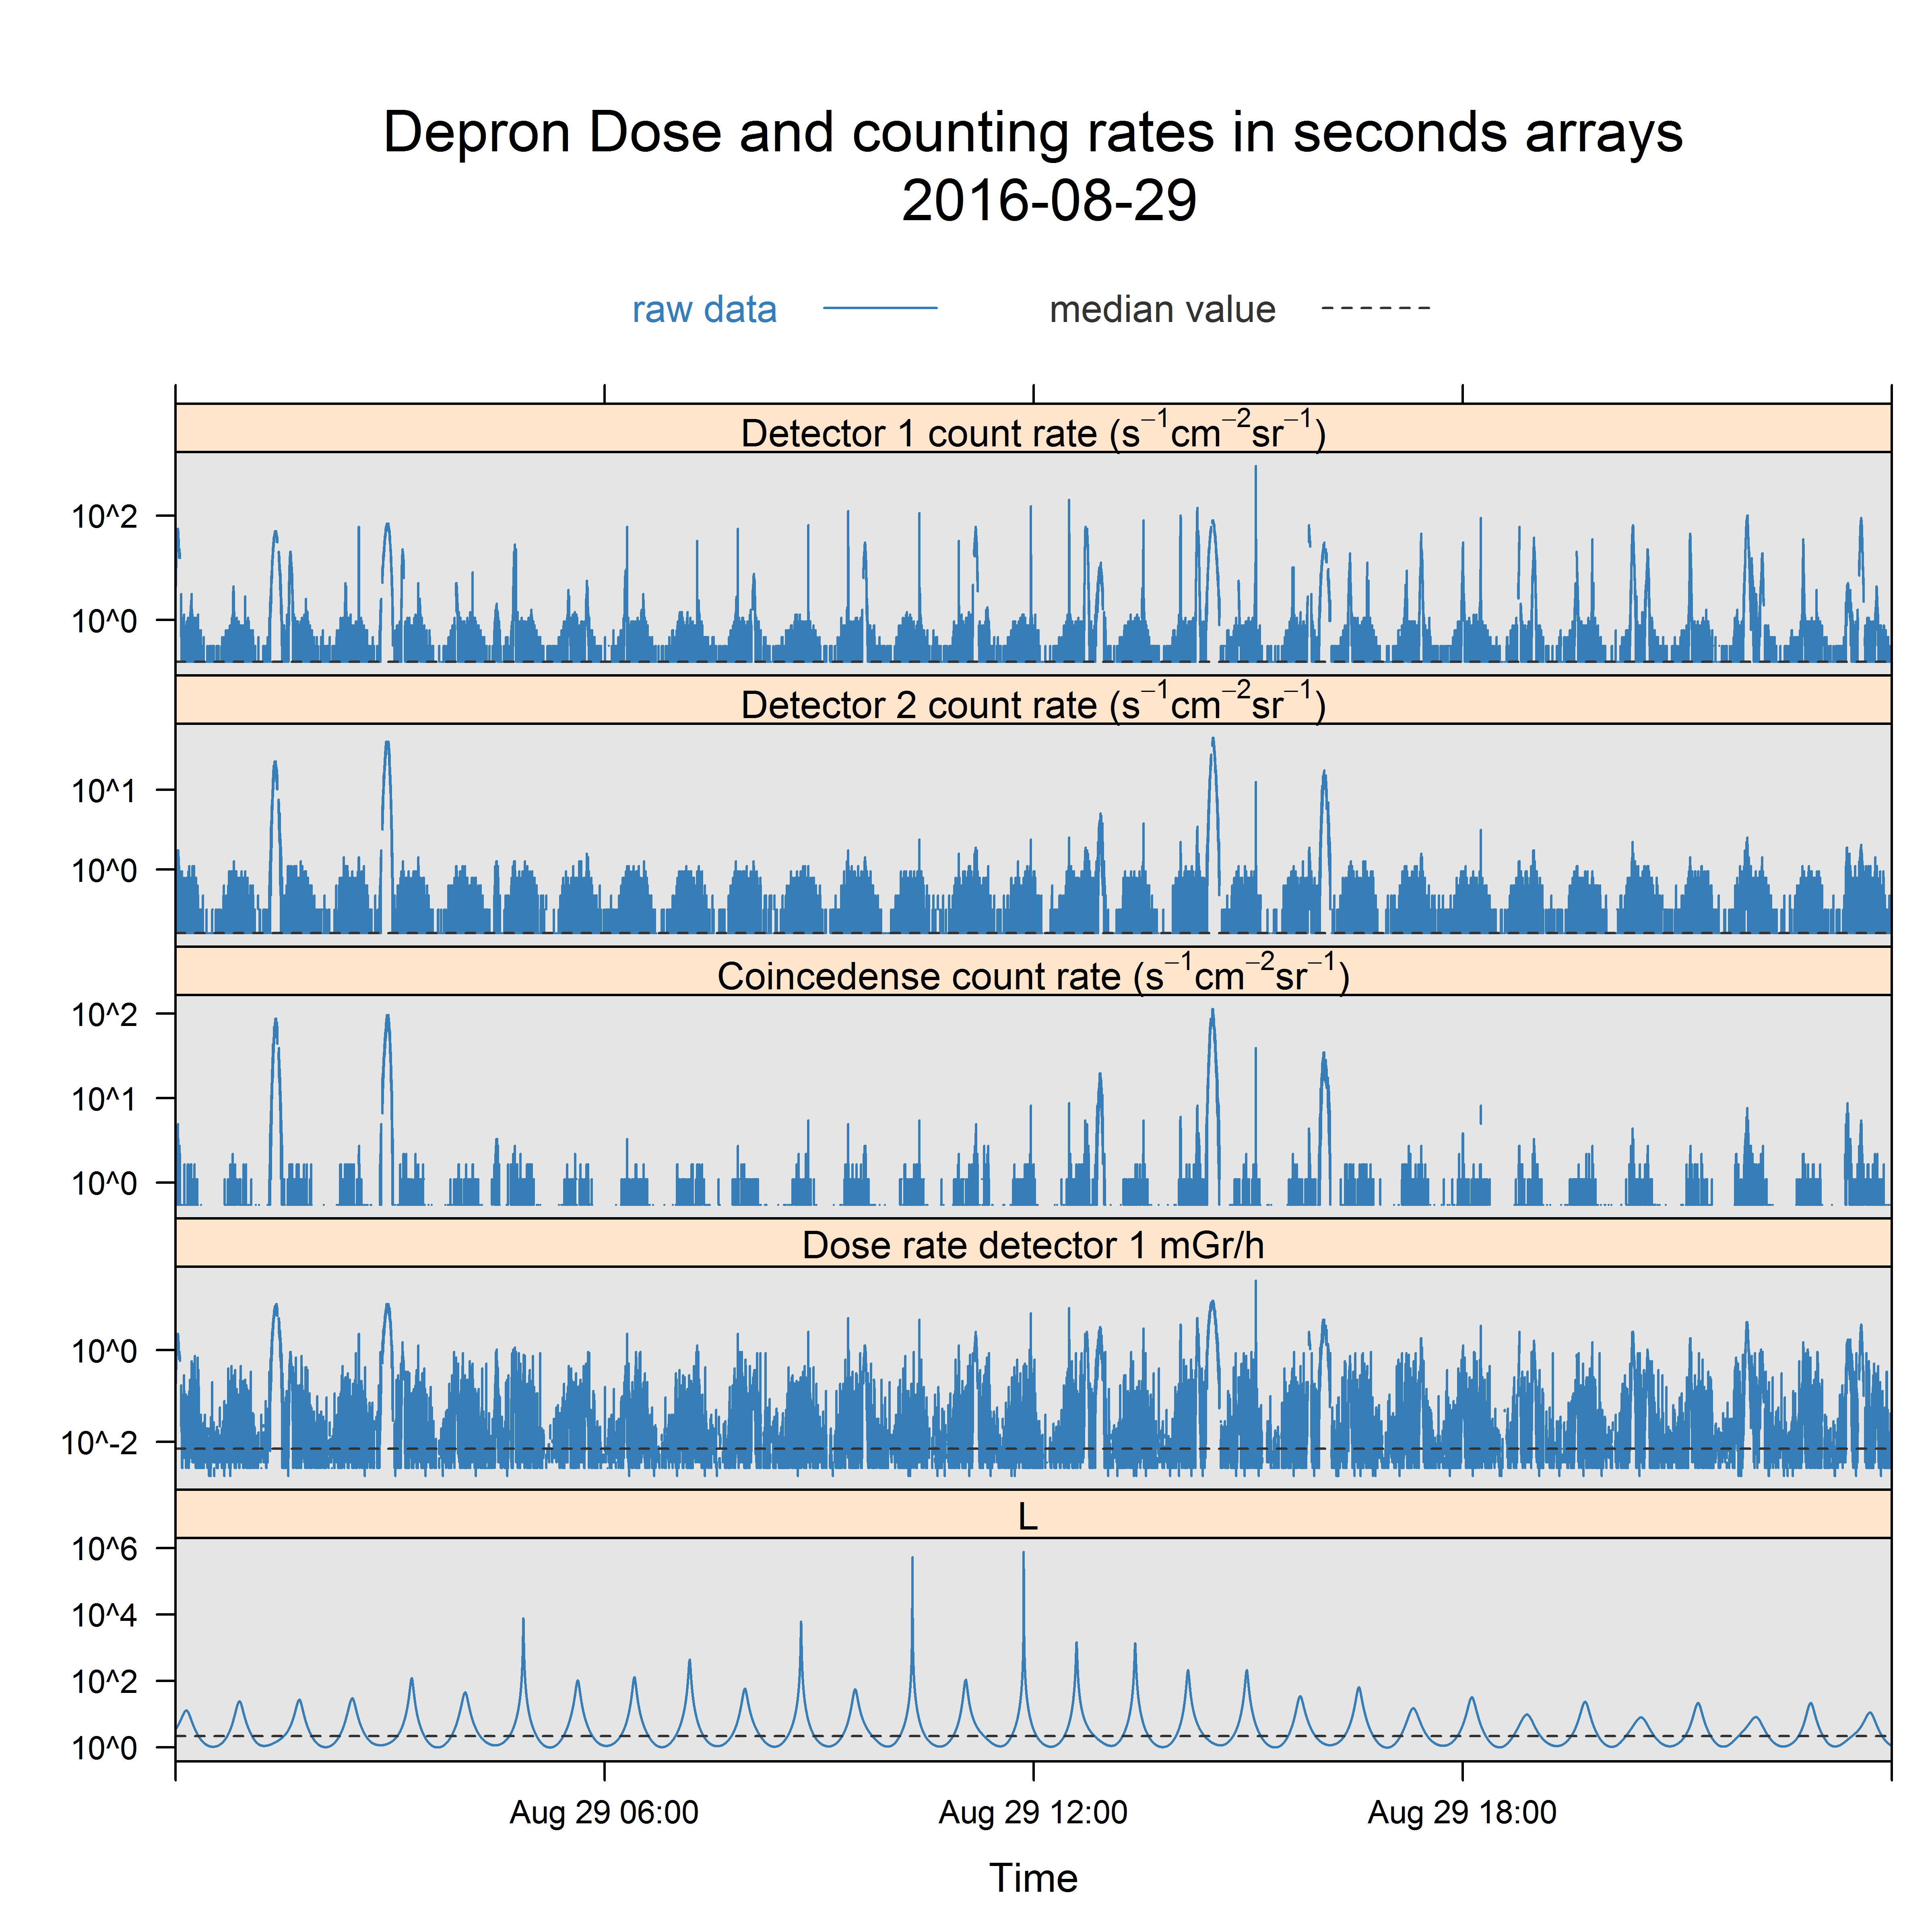
\includegraphics[width=0.5\linewidth]{images/results/depron_sec_log08-29-16}
	\caption{Временные серии в детекторах прибора.}
	\label{fig:depronseclog08-29-16}
\end{figure}

В первую очередь для каждого дня работы прибора были построены карты скоростей счета в первом детекторе \ref{sec:planetDose}.В процессе построения пространственного распределения было обнаружено расхождение меток времени  ДЭПРОН и всемирного времени. Разработанное решение проблемы привязки данных подробно рассматривается в разделе \ref{sec3.2}.

Аналогично картам были построены долготные зависимости скоростей счета в первом детекторе, эти графики позволили оперативно заметить резкие всплески потоков частиц во внешнем радиационном поясе. Также для каждого дня были построены карты скоростей счета в координатах Мак-Илвайна \cite{McIlwain1961}, рассчитанным по модели IGRF.

\section{Планетарное распределение потоков частиц, мощности дозы на высоте полета КА а также потоков нейтронов} \label{sec:planetDose}
При последующей обработке данных были построены графики географического распределения скоростей счета во всех детекторах прибора - двух полупроводниковых и двух нейтронных счетчиков. Цветовая схема для карт подобрана таким образом, чтобы максимальные значения были отображены красным цветом а минимальные синим, между конечными точками цвет изменяется по градиенту. Цветовая палитра квантована на 20 дискретных цветов. Каждому значению полученной дозы ставится в соответствие индекс в массиве цветов, который вычисляется по формуле:
\begin{equation*}
index_{color} = \begin{cases}
	8*\log{10}(N + 1)+1,  & \text{если } 8*\log{10}(N + 1) +1 < n \\
	n,  & \text{если } 8*\log{10}(N + 1) +1 \ge n
	\end{cases}
\end{equation*}
		где $ n $ -- цветность палитры, а $ N $ -- величина, подлежащая отображению.
						
% col = colr[ifelse(ceiling(8*log10(as.integer(combined.zoom$count1)+1))+1>n,
%n,
%ceiling(8*log10(as.integer(combined.zoom$count1)+1))+1)]
%
На картах 	\ref{fig:depronmap241} каждый маркер представляет результаты измерений детекторов за одну секунду. В качестве маркера выбран незакрашенный круг, так как в отличие от точки или линии он позволяет покрыть некоторую площадь на графике. Размер маркера подобран исходя из соображений заметания определенной площади, так как  при полете по орбите спутник покрывает 7,5 км каждую секунду. Маркеры частично перекрываются, особенно в полярных областях и наилучшие результаты по отображению были получены при использовании частичной прозрачности. Для простоты отображения выбрана прямоугольная проекция карты по широте и долготе, поэтому на различных широтах площадь отображаемой поверхности не искажена. Это обстоятельство таким образом лишь условно соотвествует величине траектории вдоль которой производилось измерение.
\begin{figure}[h]
	\centering
	\includegraphics[width=0.7\linewidth]{images/depronmap241}
	\caption{Карта распределения счета в первом детекторе.}
	\label{fig:depronmap241}
\end{figure}

\section{Распределения мощности дозы в области ЮАА}
Из результатов исследований НИИЯФ МГУ \cite{Lishnevskii2012} известно, что дозы,  набираемые при пролетах МКС через области аномалии являются значительными несмотря на малые участки траектории пересекающие аномалию. Аналогичная ситуация возникает и на полярной орбите, что подтверждают данные ДЭПРОН. 

В качестве примера возьмем временные серии скоростей счета и мощности дозы, полученные с ДЭПРОН для 14:30 29 Августа 2016 года \ref{fig:depronseclognew08-29-1614-24-23}. Возрастание скоростей счета и доз связано с пересечением ЮАА. Точками показаны измерения с детекторов с секундным разрешением, сплошными линиями отражено сглаживание данных треугольным фильтром.

\begin{figure}
	\centering
	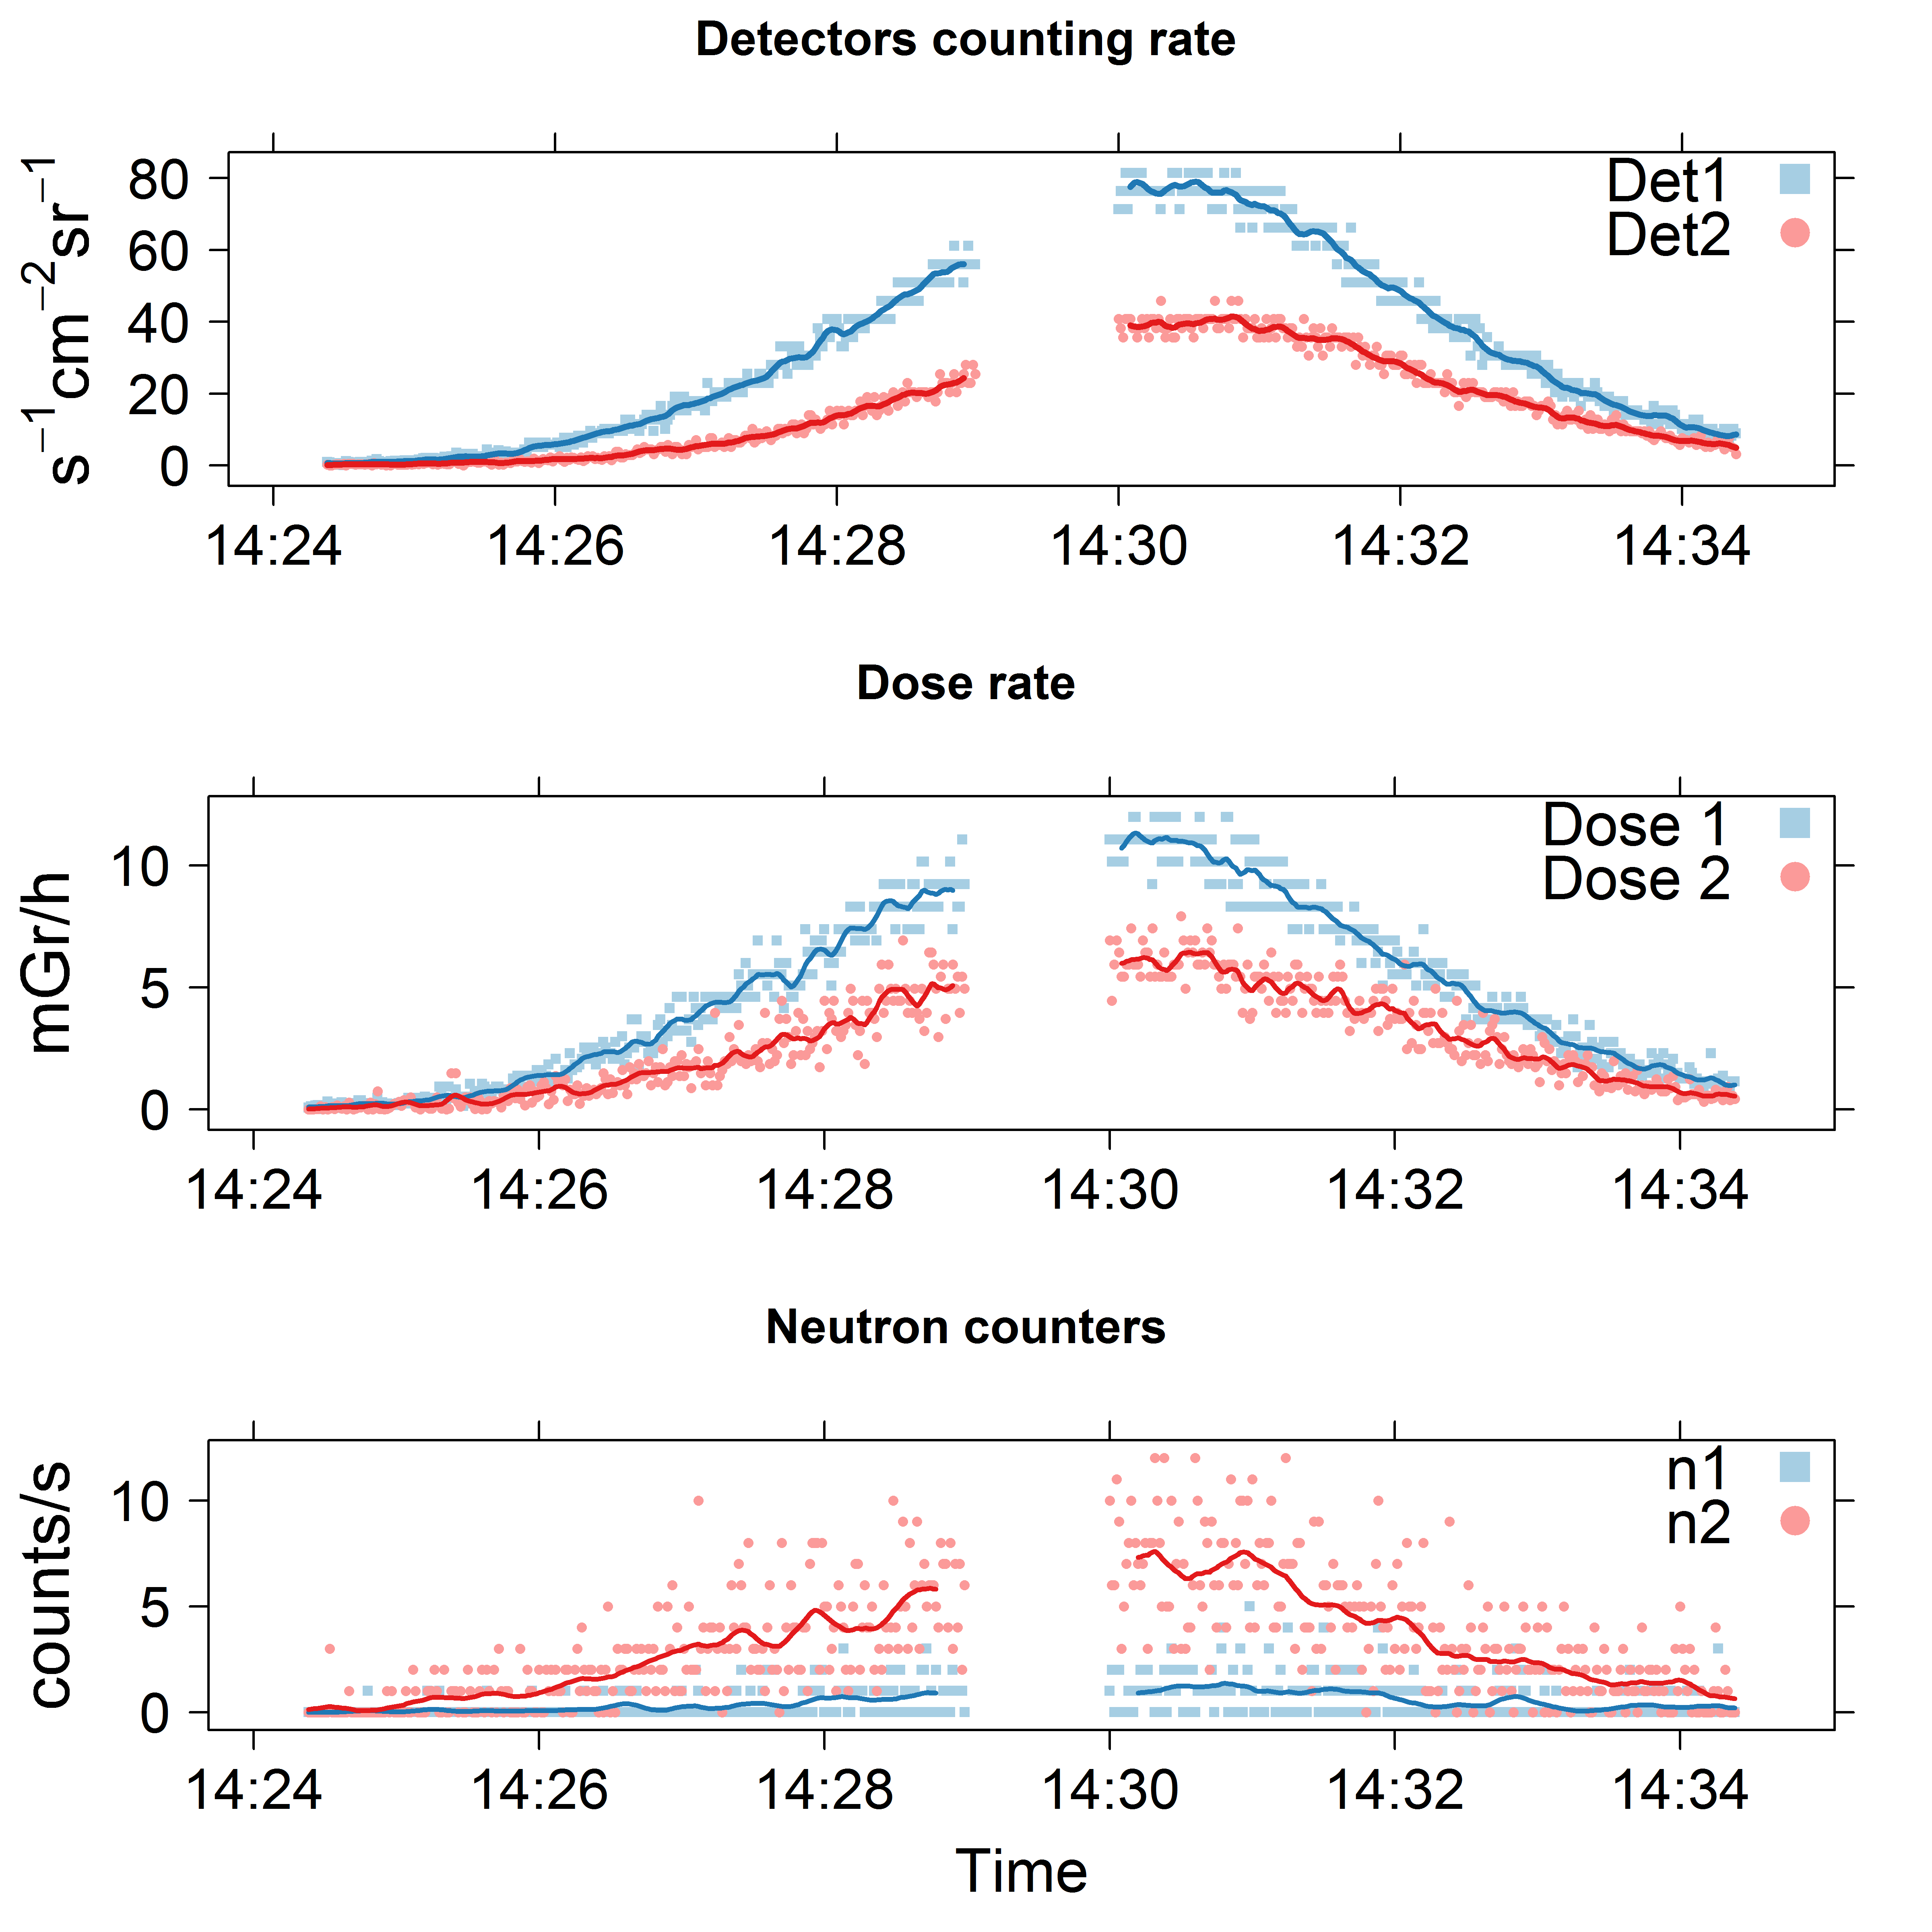
\includegraphics[width=0.5\linewidth]{images/results/depron_sec_log_new08-29-1614-24-23}
	\caption{Временные серии скоростей счета и мощности дозы при пересечении внутреннего радиационного пояса}	\label{fig:depronseclognew08-29-1614-24-23}
\end{figure}

Видно, что в данных отсутствует минута измерений 14:29, это является последствием загруженности канала передачи данных. 




\section{Распределения мощности дозы в авроральных областях}
В  данных  ДЭПРОН приполярные области отличаются высокой вариабельностью во времени и пространстве потоков частиц и соответственно доз. Были найдены и выделены возрастания скоростей счета в первом детекторе	\label{fig:depronlatmap148}, превышающие по абсолютной величине 5000 отсчетов в секунду, что соответствует более 800 с\textsuperscript{-1} см\textsuperscript{-1} стер\textsuperscript{-1}. 
\begin{figure}[h]
	\centering
	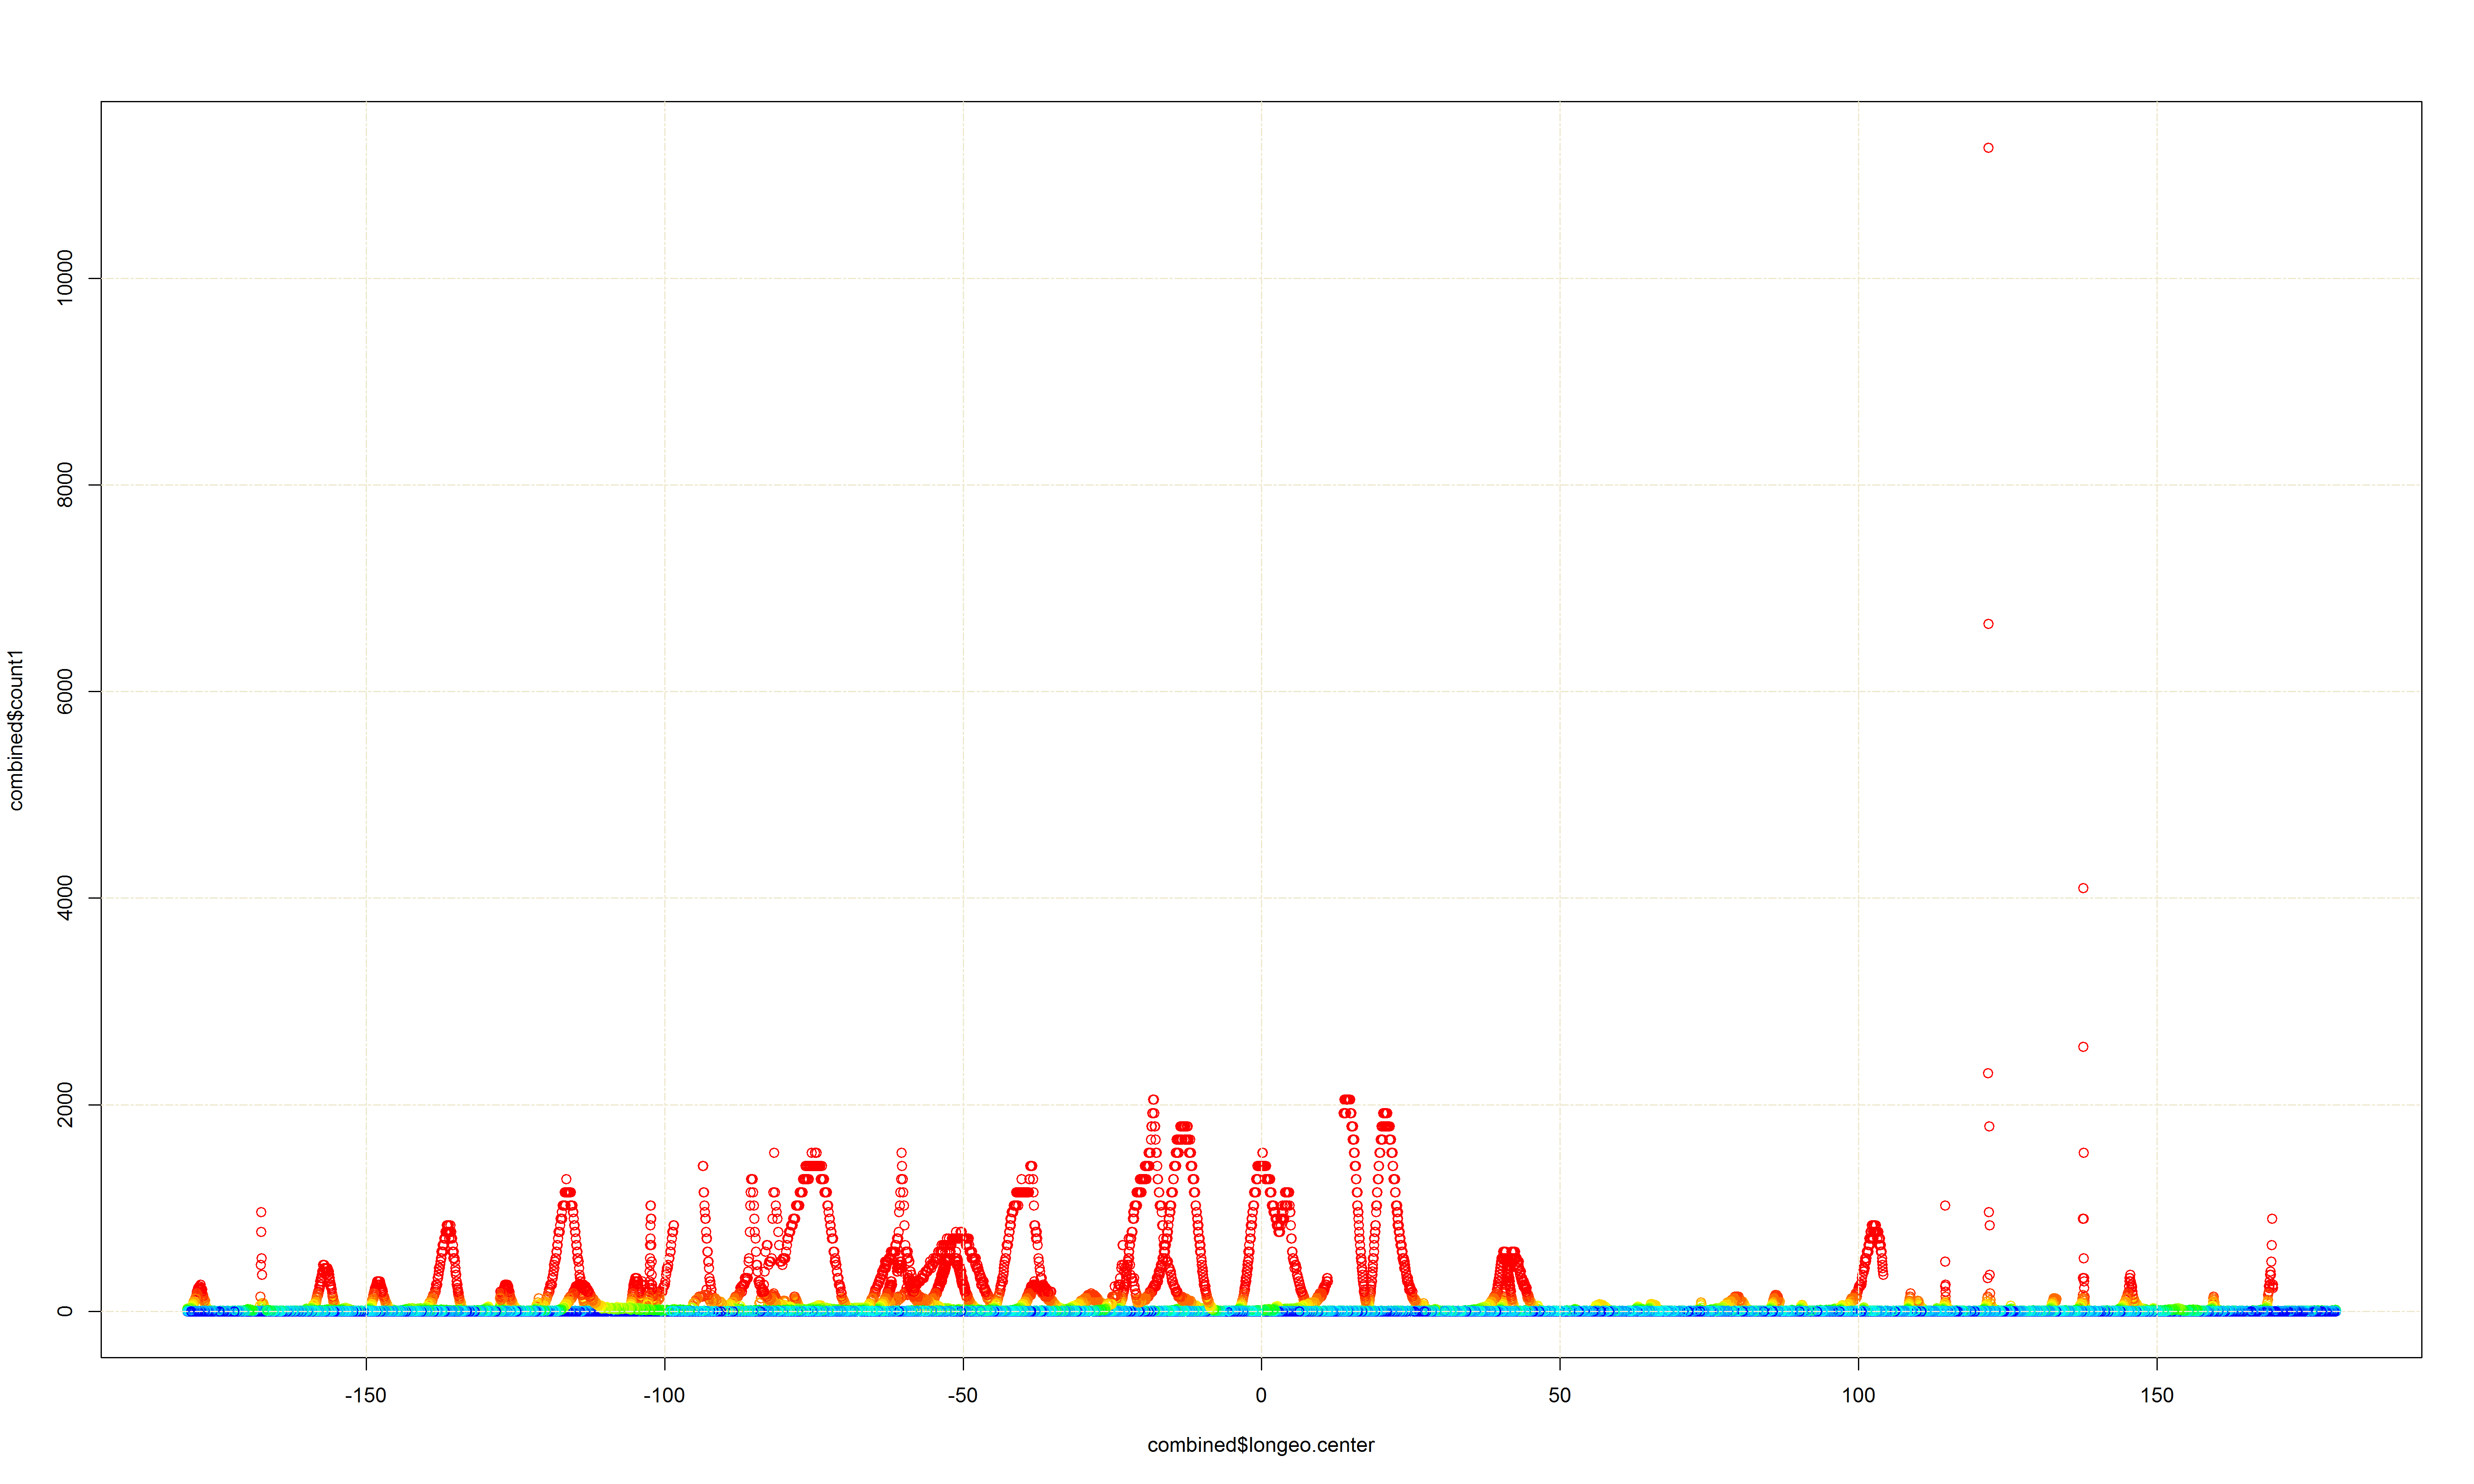
\includegraphics[width=0.8\linewidth]{images/Flash/depron_lat_map_148}
	\caption{Географическое распределение потоков заряженных частиц в первом полупроводниковом детекторе. Для наглядности счет в детекторе показан в линейном масштабе.}
	\label{fig:depronlatmap148}
\end{figure}
Величины повышенных потоков, зарегистрированных в первом полупроводниковом детекторе в среднем в 30-100 раз выше чем во втором детекторе и при одновременной регистрации в двух детекторах.
\begin{figure}[h]
	\centering
	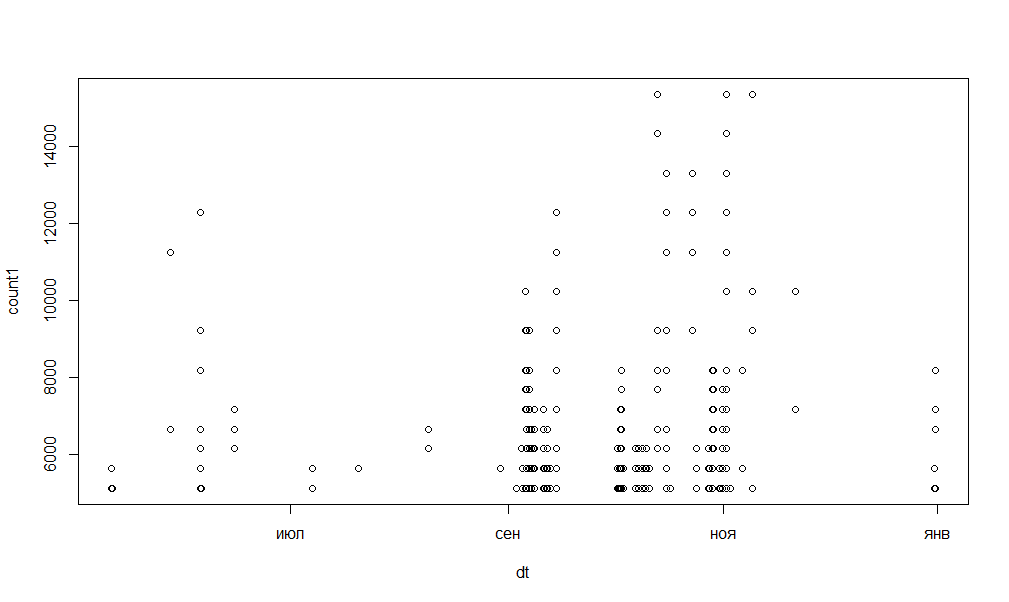
\includegraphics[width=0.7\linewidth]{images/Flash/Rplot03}
	\caption{Временное распределение зарегистрированных вспышек. Общее число выделенных вспышек за время работы прибора ДЭПРОН достигает 90.}
	\label{fig:rplot03}
\end{figure}

Учитывая, что геометрический фактор телескопа детекторов в 3 раза меньше чем геометрический фактор верхнего детектора, мы можем предположить что энергии частиц в этих потоках невысоки, поэтому большая часть частиц до второго детектора не доходит.	Для наибольших возрастаний счета отношение скоростей счета меньше и составляет один порядок и здесь энергия частиц больше. Мы наблюдаем четкое разделение по скорости счета и соотношению в верхнем и нижнем детекторах. 
\begin{figure}[h]
	\centering
	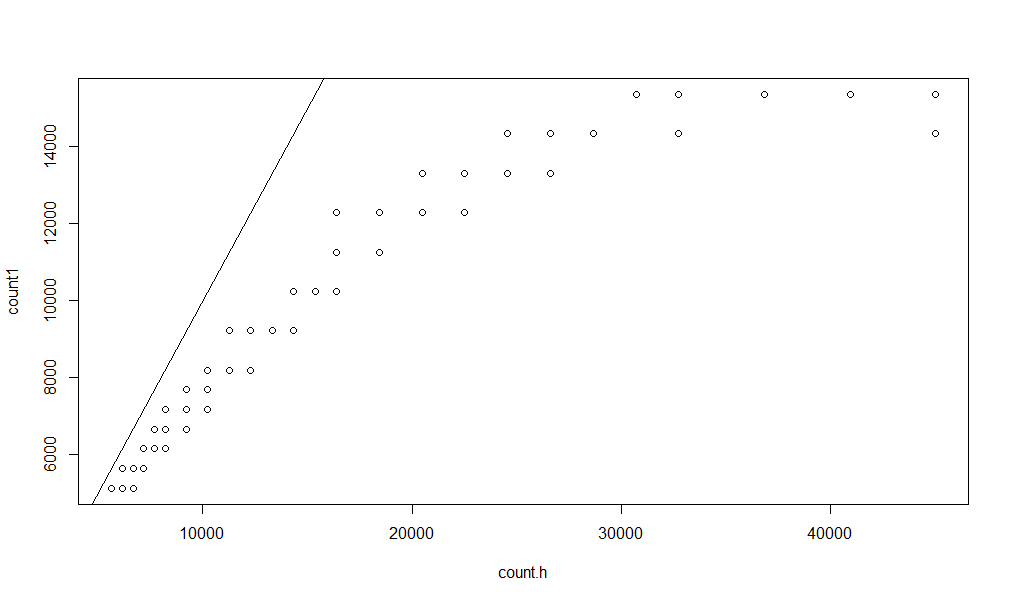
\includegraphics[width=0.7\linewidth]{images/Flash/Rplot04}
	\caption{Соотношение программного и аппаратного счетчиков для секунд, в которые регистрировались вспышки. Прямая на рисунке показывает соотношение при котором все зарегистрированные частицы обработаны программой прибора.}
	\label{fig:rplot04}
\end{figure}
Соотношение аппаратного счетчика первого детектора и программного счетчика позволяет сделать вывод, что при высоких загрузках микроконтроллер ДЭПРОН не успевает программно обработать все зарегистрированные детекторами частицы. Зависимость \ref{fig:rplot04} отношения обработанных и всех частиц практически линейна до скоростей счета 5000 за секунду, а более 10 тысяч отсчетов становиться нелинейной. В максимальных импульсах зарегистрированных за время работы ДЭПРОН, не обработано в три раза больше прерываний от частиц, чем обработано программно. Это обстоятельство помогает сделать верные поправки в большую сторону при оценке дозовых нагрузок во время вспышек. 
\begin{figure}
	\centering
	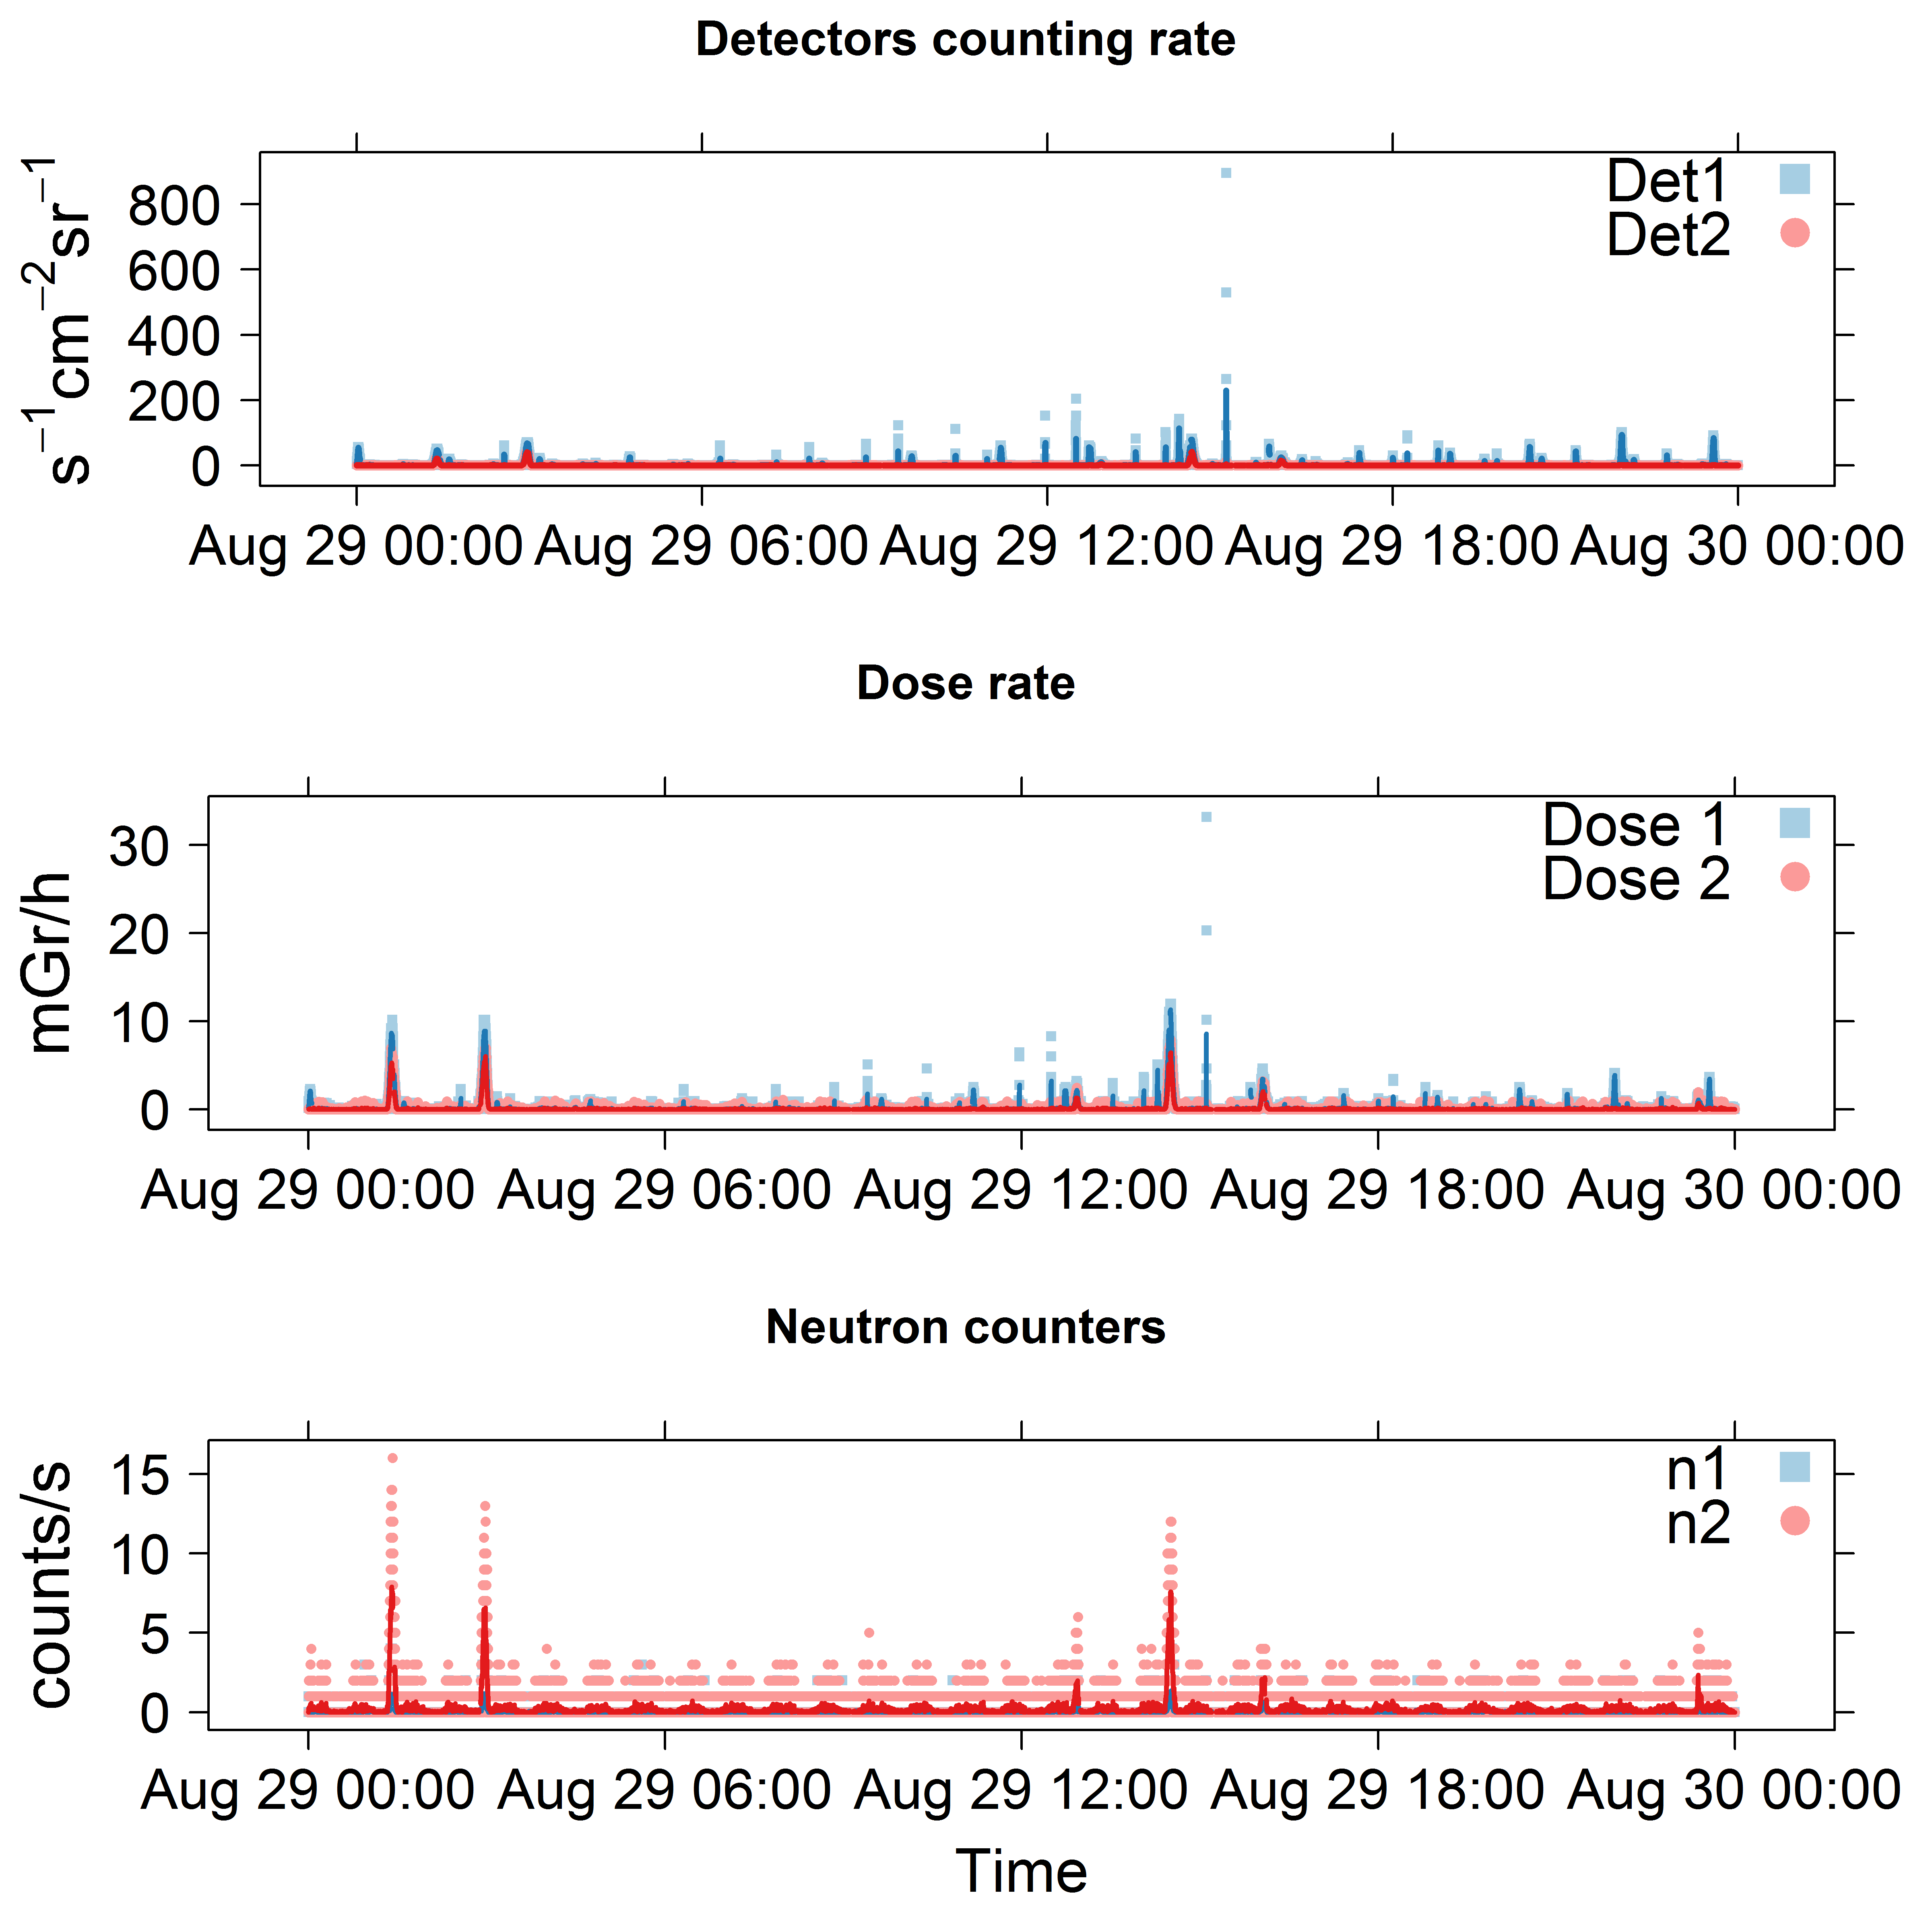
\includegraphics[width=0.7\linewidth]{images/results/depron_sec_log_new08-29-16}
	\caption{}
	\label{fig:depronseclognew08-29-16}
\end{figure}


%Рассмотреть зависимости дозы в L-B координатах разделив при этом утреннее в вечернее местное магнитное время (MLT) о наличии магнитной бури следить по индексам A(e) A(l), причем по мнению Антоновой стоит выбрать спокойный период.

%Построены зависимости B(t) для L из диапазонов от 4-5, 5-6, 6-7.



Также построены зависимости L(t) \ref{fig:l-t2016}. Для сравнения представлены результаты измерений электронов с энергиями более 2 МэВ на спутниках Van Allen \ref{fig:van-allen-lshell-crop}. 
\begin{figure}
	\centering
	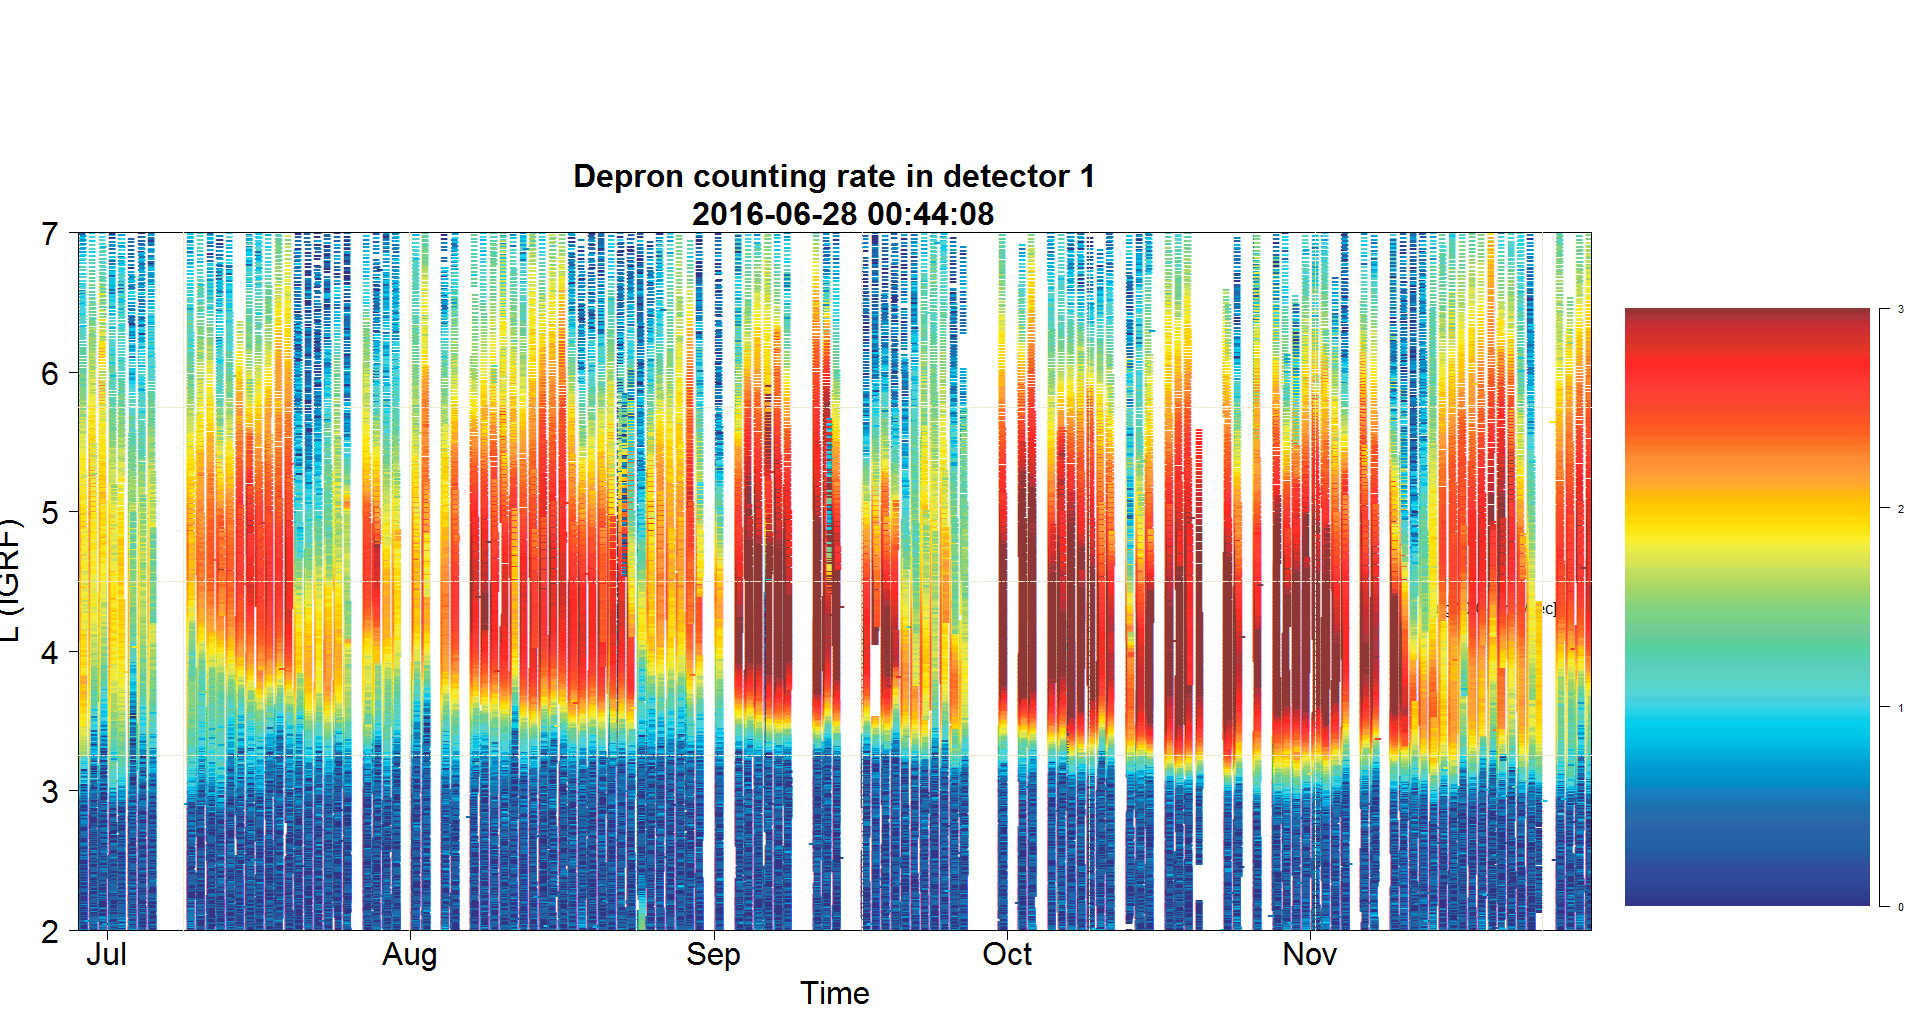
\includegraphics[width=0.9\linewidth]{images/L-t2016}
	\caption{Зависимость скорости счета в первом детекторе от времени и параметра Мак-Илвайна L.}
	\label{fig:l-t2016}
\end{figure}
\begin{figure}
	\centering		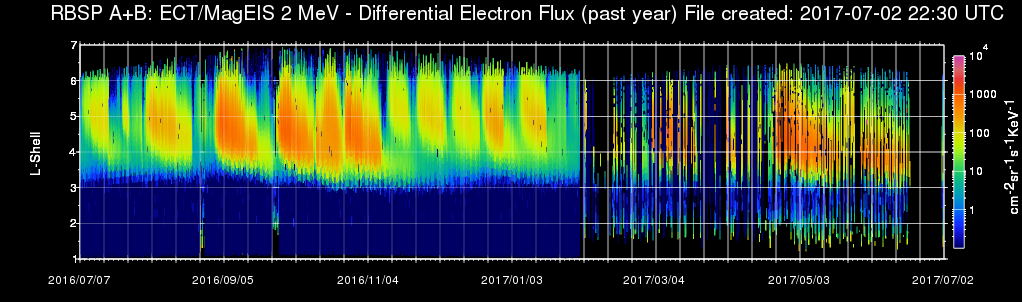
\includegraphics[width=0.7\linewidth]{../literature_repository/relelec/van-allen-lshell-crop}
	\caption{Дифференциальный поток электронов с энергией более 2 МэВ, по данным спутников RPSB A и RPSB B. По материалам: \cite{NOAA}}
	\label{fig:van-allen-lshell-crop}
\end{figure}



\begin{figure}
	\centering
	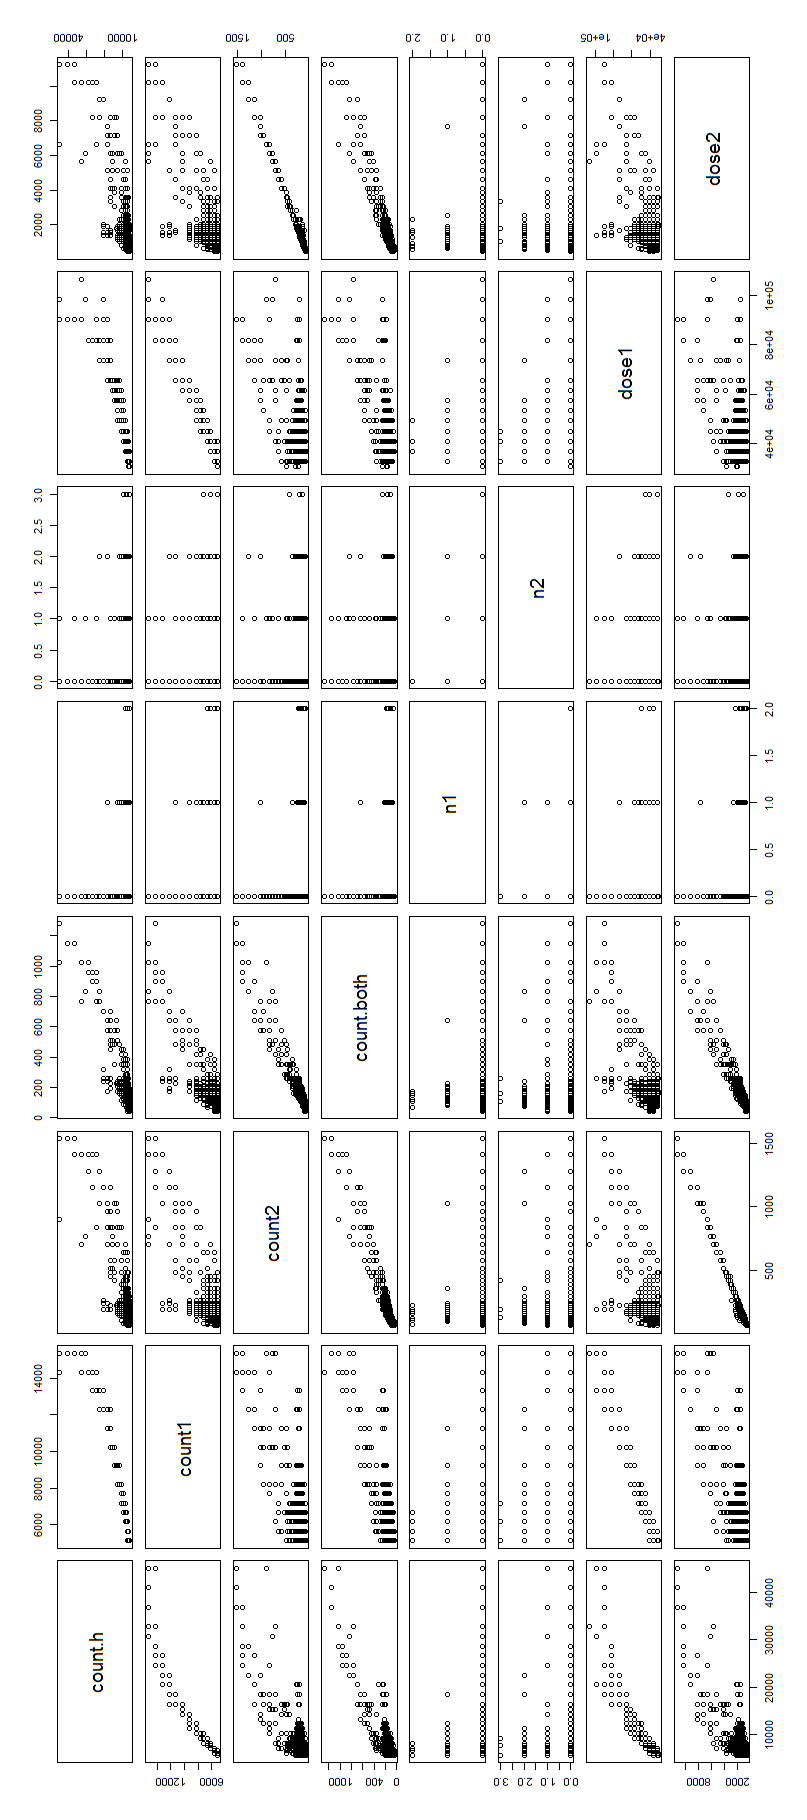
\includegraphics[width=0.7\linewidth]{images/Flash/Rplot06}
	\caption{}
	\label{fig:rplot06}
\end{figure}

\begin{figure}
	\centering
	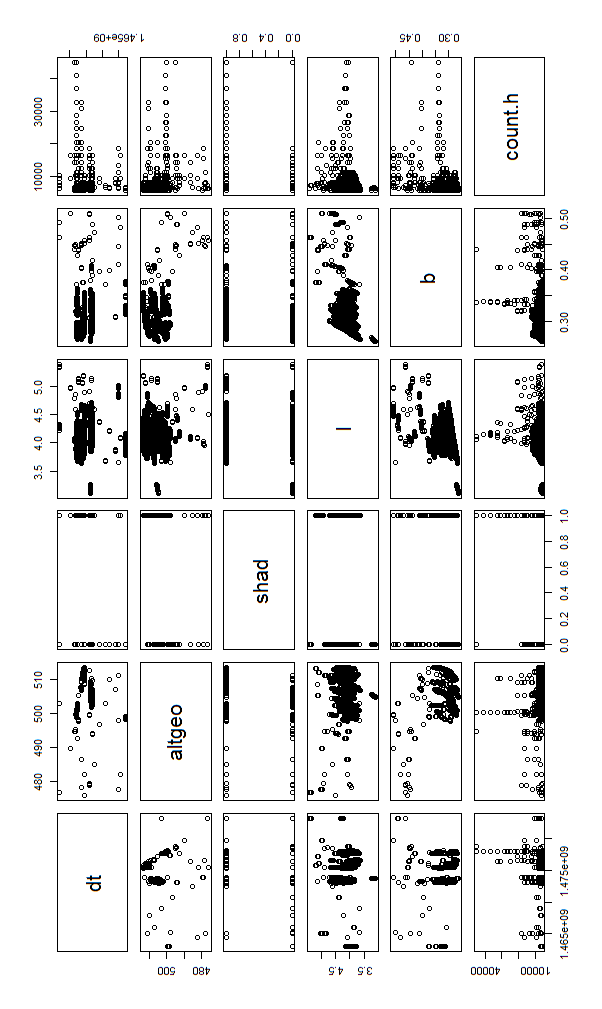
\includegraphics[width=0.7\linewidth]{images/Flash/Rplot08}
	\caption{}
	\label{fig:rplot08}
\end{figure}

\section{Распределение мощности дозы вне радиационных поясов Земли}

\section{Спектры ЛПЭ и распределение мощности эквивалентной дозы}